\PassOptionsToPackage{unicode=true}{hyperref} % options for packages loaded elsewhere
\PassOptionsToPackage{hyphens}{url}
\PassOptionsToPackage{dvipsnames,svgnames*,x11names*}{xcolor}
%
\documentclass[ignorenonframetext,]{beamer}
\usepackage{pgfpages}
\setbeamertemplate{caption}[numbered]
\setbeamertemplate{caption label separator}{: }
\setbeamercolor{caption name}{fg=normal text.fg}
\beamertemplatenavigationsymbolsempty
% Prevent slide breaks in the middle of a paragraph:
\widowpenalties 1 10000
\raggedbottom
\setbeamertemplate{part page}{
\centering
\begin{beamercolorbox}[sep=16pt,center]{part title}
  \usebeamerfont{part title}\insertpart\par
\end{beamercolorbox}
}
\setbeamertemplate{section page}{
\centering
\begin{beamercolorbox}[sep=12pt,center]{part title}
  \usebeamerfont{section title}\insertsection\par
\end{beamercolorbox}
}
\setbeamertemplate{subsection page}{
\centering
\begin{beamercolorbox}[sep=8pt,center]{part title}
  \usebeamerfont{subsection title}\insertsubsection\par
\end{beamercolorbox}
}
\AtBeginPart{
  \frame{\partpage}
}
\AtBeginSection{
  \ifbibliography
  \else
    \frame{\sectionpage}
  \fi
}
\AtBeginSubsection{
  \frame{\subsectionpage}
}
\usepackage{lmodern}
\usepackage{amssymb,amsmath}
\usepackage{ifxetex,ifluatex}
\usepackage{fixltx2e} % provides \textsubscript
\ifnum 0\ifxetex 1\fi\ifluatex 1\fi=0 % if pdftex
  \usepackage[T1]{fontenc}
  \usepackage[utf8]{inputenc}
  \usepackage{textcomp} % provides euro and other symbols
\else % if luatex or xelatex
  \usepackage{unicode-math}
  \defaultfontfeatures{Ligatures=TeX,Scale=MatchLowercase}
\fi
% use upquote if available, for straight quotes in verbatim environments
\IfFileExists{upquote.sty}{\usepackage{upquote}}{}
% use microtype if available
\IfFileExists{microtype.sty}{%
\usepackage[]{microtype}
\UseMicrotypeSet[protrusion]{basicmath} % disable protrusion for tt fonts
}{}
\IfFileExists{parskip.sty}{%
\usepackage{parskip}
}{% else
\setlength{\parindent}{0pt}
\setlength{\parskip}{6pt plus 2pt minus 1pt}
}
\usepackage{xcolor}
\usepackage{hyperref}
\hypersetup{
            pdftitle={Introduction to R Programming},
            pdfauthor={Pedro Fonseca},
            colorlinks=true,
            linkcolor=Maroon,
            filecolor=Maroon,
            citecolor=Blue,
            urlcolor=blue,
            breaklinks=true}
\urlstyle{same}  % don't use monospace font for urls
\newif\ifbibliography
\usepackage{color}
\usepackage{fancyvrb}
\newcommand{\VerbBar}{|}
\newcommand{\VERB}{\Verb[commandchars=\\\{\}]}
\DefineVerbatimEnvironment{Highlighting}{Verbatim}{commandchars=\\\{\}}
% Add ',fontsize=\small' for more characters per line
\usepackage{framed}
\definecolor{shadecolor}{RGB}{248,248,248}
\newenvironment{Shaded}{\begin{snugshade}}{\end{snugshade}}
\newcommand{\AlertTok}[1]{\textcolor[rgb]{0.94,0.16,0.16}{#1}}
\newcommand{\AnnotationTok}[1]{\textcolor[rgb]{0.56,0.35,0.01}{\textbf{\textit{#1}}}}
\newcommand{\AttributeTok}[1]{\textcolor[rgb]{0.77,0.63,0.00}{#1}}
\newcommand{\BaseNTok}[1]{\textcolor[rgb]{0.00,0.00,0.81}{#1}}
\newcommand{\BuiltInTok}[1]{#1}
\newcommand{\CharTok}[1]{\textcolor[rgb]{0.31,0.60,0.02}{#1}}
\newcommand{\CommentTok}[1]{\textcolor[rgb]{0.56,0.35,0.01}{\textit{#1}}}
\newcommand{\CommentVarTok}[1]{\textcolor[rgb]{0.56,0.35,0.01}{\textbf{\textit{#1}}}}
\newcommand{\ConstantTok}[1]{\textcolor[rgb]{0.00,0.00,0.00}{#1}}
\newcommand{\ControlFlowTok}[1]{\textcolor[rgb]{0.13,0.29,0.53}{\textbf{#1}}}
\newcommand{\DataTypeTok}[1]{\textcolor[rgb]{0.13,0.29,0.53}{#1}}
\newcommand{\DecValTok}[1]{\textcolor[rgb]{0.00,0.00,0.81}{#1}}
\newcommand{\DocumentationTok}[1]{\textcolor[rgb]{0.56,0.35,0.01}{\textbf{\textit{#1}}}}
\newcommand{\ErrorTok}[1]{\textcolor[rgb]{0.64,0.00,0.00}{\textbf{#1}}}
\newcommand{\ExtensionTok}[1]{#1}
\newcommand{\FloatTok}[1]{\textcolor[rgb]{0.00,0.00,0.81}{#1}}
\newcommand{\FunctionTok}[1]{\textcolor[rgb]{0.00,0.00,0.00}{#1}}
\newcommand{\ImportTok}[1]{#1}
\newcommand{\InformationTok}[1]{\textcolor[rgb]{0.56,0.35,0.01}{\textbf{\textit{#1}}}}
\newcommand{\KeywordTok}[1]{\textcolor[rgb]{0.13,0.29,0.53}{\textbf{#1}}}
\newcommand{\NormalTok}[1]{#1}
\newcommand{\OperatorTok}[1]{\textcolor[rgb]{0.81,0.36,0.00}{\textbf{#1}}}
\newcommand{\OtherTok}[1]{\textcolor[rgb]{0.56,0.35,0.01}{#1}}
\newcommand{\PreprocessorTok}[1]{\textcolor[rgb]{0.56,0.35,0.01}{\textit{#1}}}
\newcommand{\RegionMarkerTok}[1]{#1}
\newcommand{\SpecialCharTok}[1]{\textcolor[rgb]{0.00,0.00,0.00}{#1}}
\newcommand{\SpecialStringTok}[1]{\textcolor[rgb]{0.31,0.60,0.02}{#1}}
\newcommand{\StringTok}[1]{\textcolor[rgb]{0.31,0.60,0.02}{#1}}
\newcommand{\VariableTok}[1]{\textcolor[rgb]{0.00,0.00,0.00}{#1}}
\newcommand{\VerbatimStringTok}[1]{\textcolor[rgb]{0.31,0.60,0.02}{#1}}
\newcommand{\WarningTok}[1]{\textcolor[rgb]{0.56,0.35,0.01}{\textbf{\textit{#1}}}}
\usepackage{graphicx,grffile}
\makeatletter
\def\maxwidth{\ifdim\Gin@nat@width>\linewidth\linewidth\else\Gin@nat@width\fi}
\def\maxheight{\ifdim\Gin@nat@height>\textheight\textheight\else\Gin@nat@height\fi}
\makeatother
% Scale images if necessary, so that they will not overflow the page
% margins by default, and it is still possible to overwrite the defaults
% using explicit options in \includegraphics[width, height, ...]{}
\setkeys{Gin}{width=\maxwidth,height=\maxheight,keepaspectratio}
\setlength{\emergencystretch}{3em}  % prevent overfull lines
\providecommand{\tightlist}{%
  \setlength{\itemsep}{0pt}\setlength{\parskip}{0pt}}
\setcounter{secnumdepth}{0}

% set default figure placement to htbp
\makeatletter
\def\fps@figure{htbp}
\makeatother


\title{Introduction to R Programming}
\providecommand{\subtitle}[1]{}
\subtitle{Factors}
\author{Pedro Fonseca}
\date{10 May 2020}

\begin{document}
\frame{\titlepage}

\begin{frame}{What are factors?}
\protect\hypertarget{what-are-factors}{}

\begin{itemize}
\item
  A factor is a vector that can contain only predefined values
\item
  Factors are used to represent categorical data
\end{itemize}

\end{frame}

\begin{frame}{Categorical variables}
\protect\hypertarget{categorical-variables}{}

\begin{itemize}
\item
  Categorical variables have a limited and known set of possible
  outcomes
\item
  Categorical variables typically qualitative
\end{itemize}

\end{frame}

\begin{frame}{Categorical variables}
\protect\hypertarget{categorical-variables-1}{}

Examples:

\begin{itemize}
\item
  flip of a coin (heads or tails)
\item
  size of a shirt (S, M, L, XL, XXL, XXXL)
\item
  marital status (single, married, divorced, widowed)
\item
  credit rating (very bad, bad, average, good, excellent)
\item
  school grades (A, B, C, D, E, F)
\end{itemize}

\end{frame}

\begin{frame}{Categorical variables}
\protect\hypertarget{categorical-variables-2}{}

\begin{figure}
\centering
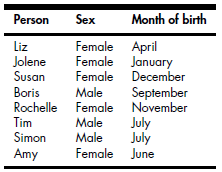
\includegraphics{figures/dataset.png}
\caption{Dataset with categorical variables}
\end{figure}

\end{frame}

\begin{frame}{More about factors}
\protect\hypertarget{more-about-factors}{}

\begin{itemize}
\item
  Factors are built on top of integers
\item
  They come with two attributes:

  \begin{itemize}
  \item
    Levels, which define the set of allowed values
  \item
    Their own class, ``factor'', which makes them behave differently
    from regular integers
  \end{itemize}
\end{itemize}

\end{frame}

\begin{frame}[fragile]{Creating a factor}
\protect\hypertarget{creating-a-factor}{}

Let's start with a character vector:

\begin{Shaded}
\begin{Highlighting}[]
\NormalTok{blood <-}\StringTok{ }\KeywordTok{c}\NormalTok{(}\StringTok{"B"}\NormalTok{, }\StringTok{"AB"}\NormalTok{, }\StringTok{"O"}\NormalTok{, }\StringTok{"A"}\NormalTok{, }\StringTok{"O"}\NormalTok{, }\StringTok{"O"}\NormalTok{, }\StringTok{"A"}\NormalTok{) }

\NormalTok{blood}
\end{Highlighting}
\end{Shaded}

\begin{verbatim}
## [1] "B"  "AB" "O"  "A"  "O"  "O"  "A"
\end{verbatim}

\end{frame}

\begin{frame}[fragile]{Creating a factor}
\protect\hypertarget{creating-a-factor-1}{}

The \texttt{factor} function encodes a vector as a factor:

\begin{Shaded}
\begin{Highlighting}[]
\NormalTok{blood_factor <-}\StringTok{ }\KeywordTok{factor}\NormalTok{(blood) }

\NormalTok{blood_factor}
\end{Highlighting}
\end{Shaded}

\begin{verbatim}
## [1] B  AB O  A  O  O  A 
## Levels: A AB B O
\end{verbatim}

Note that R sorts the levels alphabetically

\end{frame}

\begin{frame}[fragile]{Creating a factor}
\protect\hypertarget{creating-a-factor-2}{}

\begin{Shaded}
\begin{Highlighting}[]
\KeywordTok{levels}\NormalTok{(blood_factor)}
\end{Highlighting}
\end{Shaded}

\begin{verbatim}
## [1] "A"  "AB" "B"  "O"
\end{verbatim}

\begin{Shaded}
\begin{Highlighting}[]
\KeywordTok{typeof}\NormalTok{(blood_factor)}
\end{Highlighting}
\end{Shaded}

\begin{verbatim}
## [1] "integer"
\end{verbatim}

\begin{Shaded}
\begin{Highlighting}[]
\KeywordTok{class}\NormalTok{(blood_factor)}
\end{Highlighting}
\end{Shaded}

\begin{verbatim}
## [1] "factor"
\end{verbatim}

\end{frame}

\begin{frame}[fragile]{Creating a factor}
\protect\hypertarget{creating-a-factor-3}{}

When creating a factor, we can set the ordering of the levels:

\begin{Shaded}
\begin{Highlighting}[]
\NormalTok{blood_factor}
\end{Highlighting}
\end{Shaded}

\begin{verbatim}
## [1] B  AB O  A  O  O  A 
## Levels: A AB B O
\end{verbatim}

\begin{Shaded}
\begin{Highlighting}[]
\NormalTok{blood_factor2 <-}\StringTok{ }\KeywordTok{factor}\NormalTok{(blood,}
                    \DataTypeTok{levels =} \KeywordTok{c}\NormalTok{(}\StringTok{"O"}\NormalTok{, }\StringTok{"A"}\NormalTok{, }\StringTok{"B"}\NormalTok{, }\StringTok{"AB"}\NormalTok{))}
\NormalTok{blood_factor2}
\end{Highlighting}
\end{Shaded}

\begin{verbatim}
## [1] B  AB O  A  O  O  A 
## Levels: O A B AB
\end{verbatim}

\end{frame}

\begin{frame}[fragile]{Order levels differently}
\protect\hypertarget{order-levels-differently}{}

We can modify the ordering of the levels of an existing factor:

\begin{Shaded}
\begin{Highlighting}[]
\NormalTok{blood_factor}
\end{Highlighting}
\end{Shaded}

\begin{verbatim}
## [1] B  AB O  A  O  O  A 
## Levels: A AB B O
\end{verbatim}

\begin{Shaded}
\begin{Highlighting}[]
\KeywordTok{factor}\NormalTok{(blood_factor, }\DataTypeTok{levels =} \KeywordTok{c}\NormalTok{(}\StringTok{"O"}\NormalTok{, }\StringTok{"A"}\NormalTok{, }\StringTok{"B"}\NormalTok{, }\StringTok{"AB"}\NormalTok{))}
\end{Highlighting}
\end{Shaded}

\begin{verbatim}
## [1] B  AB O  A  O  O  A 
## Levels: O A B AB
\end{verbatim}

\end{frame}

\begin{frame}[fragile]{Order levels differently}
\protect\hypertarget{order-levels-differently-1}{}

\texttt{Relevel} re-orders the levels of a factor so that the level
specified by \texttt{ref} is the first level:

\begin{Shaded}
\begin{Highlighting}[]
\NormalTok{blood_factor}
\end{Highlighting}
\end{Shaded}

\begin{verbatim}
## [1] B  AB O  A  O  O  A 
## Levels: A AB B O
\end{verbatim}

\begin{Shaded}
\begin{Highlighting}[]
\KeywordTok{relevel}\NormalTok{(blood_factor, }\DataTypeTok{ref =} \StringTok{"O"}\NormalTok{)}
\end{Highlighting}
\end{Shaded}

\begin{verbatim}
## [1] B  AB O  A  O  O  A 
## Levels: O A AB B
\end{verbatim}

\end{frame}

\begin{frame}[fragile]{Order levels differently}
\protect\hypertarget{order-levels-differently-2}{}

With \texttt{rev} we can reverse the ordering of the levels of a factor:

\begin{Shaded}
\begin{Highlighting}[]
\NormalTok{blood_factor}
\end{Highlighting}
\end{Shaded}

\begin{verbatim}
## [1] B  AB O  A  O  O  A 
## Levels: A AB B O
\end{verbatim}

\begin{Shaded}
\begin{Highlighting}[]
\KeywordTok{factor}\NormalTok{(blood_factor, }
  \DataTypeTok{levels =} \KeywordTok{rev}\NormalTok{(}\KeywordTok{levels}\NormalTok{(blood_factor)))}
\end{Highlighting}
\end{Shaded}

\begin{verbatim}
## [1] B  AB O  A  O  O  A 
## Levels: O B AB A
\end{verbatim}

\end{frame}

\begin{frame}[fragile]{The internal structure of a factor}
\protect\hypertarget{the-internal-structure-of-a-factor}{}

The \texttt{str} function displays the internal structure of an object:

\begin{Shaded}
\begin{Highlighting}[]
\NormalTok{blood_factor}
\end{Highlighting}
\end{Shaded}

\begin{verbatim}
## [1] B  AB O  A  O  O  A 
## Levels: A AB B O
\end{verbatim}

\begin{Shaded}
\begin{Highlighting}[]
\KeywordTok{str}\NormalTok{(blood_factor)}
\end{Highlighting}
\end{Shaded}

\begin{verbatim}
##  Factor w/ 4 levels "A","AB","B","O": 3 2 4 1 4 4 1
\end{verbatim}

\begin{itemize}
\item
  Note that the values are stored as integers!
\item
  The levels are just a set of character values to print when the factor
  is displayed
\end{itemize}

\end{frame}

\begin{frame}[fragile]{The internal structure of a factor}
\protect\hypertarget{the-internal-structure-of-a-factor-1}{}

\begin{Shaded}
\begin{Highlighting}[]
\NormalTok{blood_factor2}
\end{Highlighting}
\end{Shaded}

\begin{verbatim}
## [1] B  AB O  A  O  O  A 
## Levels: O A B AB
\end{verbatim}

\begin{Shaded}
\begin{Highlighting}[]
\KeywordTok{str}\NormalTok{(blood_factor2)}
\end{Highlighting}
\end{Shaded}

\begin{verbatim}
##  Factor w/ 4 levels "O","A","B","AB": 3 4 1 2 1 1 2
\end{verbatim}

\end{frame}

\begin{frame}[fragile]{Invalid factor levels}
\protect\hypertarget{invalid-factor-levels}{}

\begin{Shaded}
\begin{Highlighting}[]
\NormalTok{blood_factor}
\end{Highlighting}
\end{Shaded}

\begin{verbatim}
## [1] B  AB O  A  O  O  A 
## Levels: A AB B O
\end{verbatim}

\begin{Shaded}
\begin{Highlighting}[]
\NormalTok{blood_factor[}\DecValTok{3}\NormalTok{] <-}\StringTok{ "C"}
\end{Highlighting}
\end{Shaded}

\begin{Shaded}
\begin{Highlighting}[]
\NormalTok{blood_factor}
\end{Highlighting}
\end{Shaded}

\begin{verbatim}
## [1] B    AB   <NA> A    O    O    A   
## Levels: A AB B O
\end{verbatim}

\end{frame}

\begin{frame}[fragile]{Table a factor}
\protect\hypertarget{table-a-factor}{}

How many people there are with each type of blood?

\begin{Shaded}
\begin{Highlighting}[]
\KeywordTok{table}\NormalTok{(blood_factor)}
\end{Highlighting}
\end{Shaded}

\begin{verbatim}
## blood_factor
##  A AB  B  O 
##  2  1  1  2
\end{verbatim}

\begin{Shaded}
\begin{Highlighting}[]
\KeywordTok{table}\NormalTok{(blood_factor2)}
\end{Highlighting}
\end{Shaded}

\begin{verbatim}
## blood_factor2
##  O  A  B AB 
##  3  2  1  1
\end{verbatim}

\end{frame}

\begin{frame}[fragile]{Renaming factor levels}
\protect\hypertarget{renaming-factor-levels}{}

\begin{Shaded}
\begin{Highlighting}[]
\NormalTok{blood_factor2 }
\end{Highlighting}
\end{Shaded}

\begin{verbatim}
## [1] B  AB O  A  O  O  A 
## Levels: O A B AB
\end{verbatim}

\begin{Shaded}
\begin{Highlighting}[]
\KeywordTok{levels}\NormalTok{(blood_factor2) <-}\StringTok{ }\KeywordTok{c}\NormalTok{(}\StringTok{"BT_O"}\NormalTok{, }\StringTok{"BT_A"}\NormalTok{, }\StringTok{"BT_B"}\NormalTok{,}
                           \StringTok{"BT_AB"}\NormalTok{)}
\NormalTok{blood_factor2}
\end{Highlighting}
\end{Shaded}

\begin{verbatim}
## [1] BT_B  BT_AB BT_O  BT_A  BT_O  BT_O  BT_A 
## Levels: BT_O BT_A BT_B BT_AB
\end{verbatim}

\end{frame}

\begin{frame}{Levels and labels}
\protect\hypertarget{levels-and-labels}{}

\begin{itemize}
\item
  Levels are input (alphabetic order by default)
\item
  Labels are associated to levels and control how they are displayed in
  the output
\end{itemize}

\end{frame}

\begin{frame}[fragile]{Levels and labels}
\protect\hypertarget{levels-and-labels-1}{}

\begin{Shaded}
\begin{Highlighting}[]
\NormalTok{blood <-}\StringTok{ }\KeywordTok{c}\NormalTok{(}\StringTok{"B"}\NormalTok{, }\StringTok{"AB"}\NormalTok{, }\StringTok{"O"}\NormalTok{, }\StringTok{"A"}\NormalTok{, }\StringTok{"O"}\NormalTok{, }\StringTok{"O"}\NormalTok{, }\StringTok{"A"}\NormalTok{, }\StringTok{"B"}\NormalTok{) }
\KeywordTok{factor}\NormalTok{(blood)}
\end{Highlighting}
\end{Shaded}

\begin{verbatim}
## [1] B  AB O  A  O  O  A  B 
## Levels: A AB B O
\end{verbatim}

\begin{Shaded}
\begin{Highlighting}[]
\KeywordTok{factor}\NormalTok{(blood, }
         \DataTypeTok{labels =} \KeywordTok{c}\NormalTok{(}\StringTok{"BT_A"}\NormalTok{, }\StringTok{"BT_AB"}\NormalTok{, }\StringTok{"BT_B"}\NormalTok{, }\StringTok{"BT_O"}\NormalTok{))}
\end{Highlighting}
\end{Shaded}

\begin{verbatim}
## [1] BT_B  BT_AB BT_O  BT_A  BT_O  BT_O  BT_A  BT_B 
## Levels: BT_A BT_AB BT_B BT_O
\end{verbatim}

\end{frame}

\begin{frame}[fragile]{Levels and labels}
\protect\hypertarget{levels-and-labels-2}{}

\begin{Shaded}
\begin{Highlighting}[]
\KeywordTok{factor}\NormalTok{(blood)}
\end{Highlighting}
\end{Shaded}

\begin{verbatim}
## [1] B  AB O  A  O  O  A  B 
## Levels: A AB B O
\end{verbatim}

\begin{Shaded}
\begin{Highlighting}[]
\KeywordTok{factor}\NormalTok{(blood,}
         \DataTypeTok{levels =} \KeywordTok{c}\NormalTok{(}\StringTok{"O"}\NormalTok{, }\StringTok{"A"}\NormalTok{, }\StringTok{"B"}\NormalTok{, }\StringTok{"AB"}\NormalTok{),}
         \DataTypeTok{labels =} \KeywordTok{c}\NormalTok{(}\StringTok{"BT_O"}\NormalTok{, }\StringTok{"BT_A"}\NormalTok{, }\StringTok{"BT_B"}\NormalTok{, }\StringTok{"BT_AB"}\NormalTok{))}
\end{Highlighting}
\end{Shaded}

\begin{verbatim}
## [1] BT_B  BT_AB BT_O  BT_A  BT_O  BT_O  BT_A  BT_B 
## Levels: BT_O BT_A BT_B BT_AB
\end{verbatim}

\end{frame}

\begin{frame}[fragile]{Labels}
\protect\hypertarget{labels}{}

Duplicated values in \texttt{labels} can be used to map different values
of the factor to the same level:

\begin{Shaded}
\begin{Highlighting}[]
\KeywordTok{factor}\NormalTok{(blood)}
\end{Highlighting}
\end{Shaded}

\begin{verbatim}
## [1] B  AB O  A  O  O  A  B 
## Levels: A AB B O
\end{verbatim}

\begin{Shaded}
\begin{Highlighting}[]
\KeywordTok{factor}\NormalTok{(blood,}
         \DataTypeTok{levels =} \KeywordTok{c}\NormalTok{(}\StringTok{"O"}\NormalTok{, }\StringTok{"A"}\NormalTok{, }\StringTok{"B"}\NormalTok{, }\StringTok{"AB"}\NormalTok{),}
         \DataTypeTok{labels =} \KeywordTok{c}\NormalTok{(}\StringTok{"BT_O"}\NormalTok{, }\StringTok{"BT_A"}\NormalTok{, }\StringTok{"BT_B"}\NormalTok{, }\StringTok{"BT_A"}\NormalTok{))}
\end{Highlighting}
\end{Shaded}

\begin{verbatim}
## [1] BT_B BT_A BT_O BT_A BT_O BT_O BT_A BT_B
## Levels: BT_O BT_A BT_B
\end{verbatim}

\end{frame}

\begin{frame}[fragile]{Nominal versus ordinal factors}
\protect\hypertarget{nominal-versus-ordinal-factors}{}

\begin{Shaded}
\begin{Highlighting}[]
\NormalTok{blood <-}\StringTok{ }\KeywordTok{c}\NormalTok{(}\StringTok{"B"}\NormalTok{, }\StringTok{"AB"}\NormalTok{, }\StringTok{"O"}\NormalTok{, }\StringTok{"A"}\NormalTok{, }\StringTok{"O"}\NormalTok{, }\StringTok{"O"}\NormalTok{, }\StringTok{"A"}\NormalTok{, }\StringTok{"B"}\NormalTok{) }
\NormalTok{blood_factor <-}\StringTok{ }\KeywordTok{factor}\NormalTok{(blood)}

\NormalTok{blood_factor[}\DecValTok{1}\NormalTok{] }\OperatorTok{<}\StringTok{ }\NormalTok{blood_factor[}\DecValTok{2}\NormalTok{]}
\end{Highlighting}
\end{Shaded}

\begin{verbatim}
## [1] NA
\end{verbatim}

This logical comparison is not meaningful, since the factor is not
ordered

\end{frame}

\begin{frame}[fragile]{Nominal versus ordinal factors}
\protect\hypertarget{nominal-versus-ordinal-factors-1}{}

Let's build an ordered factor:

\begin{Shaded}
\begin{Highlighting}[]
\NormalTok{tshirt <-}\StringTok{ }\KeywordTok{c}\NormalTok{(}\StringTok{"M"}\NormalTok{, }\StringTok{"L"}\NormalTok{, }\StringTok{"S"}\NormalTok{, }\StringTok{"S"}\NormalTok{, }\StringTok{"L"}\NormalTok{, }\StringTok{"M"}\NormalTok{, }\StringTok{"L"}\NormalTok{, }\StringTok{"M"}\NormalTok{)}

\NormalTok{tshirt_factor <-}\StringTok{ }\KeywordTok{factor}\NormalTok{(tshirt, }
                        \DataTypeTok{ordered =} \OtherTok{TRUE}\NormalTok{, }
                        \DataTypeTok{levels =} \KeywordTok{c}\NormalTok{(}\StringTok{"S"}\NormalTok{, }\StringTok{"M"}\NormalTok{, }\StringTok{"L"}\NormalTok{))}

\NormalTok{tshirt_factor}
\end{Highlighting}
\end{Shaded}

\begin{verbatim}
## [1] M L S S L M L M
## Levels: S < M < L
\end{verbatim}

\end{frame}

\begin{frame}[fragile]{Nominal versus ordinal factors}
\protect\hypertarget{nominal-versus-ordinal-factors-2}{}

\begin{Shaded}
\begin{Highlighting}[]
\NormalTok{tshirt_factor[}\DecValTok{1}\NormalTok{] }\OperatorTok{<}\StringTok{ }\NormalTok{tshirt_factor[}\DecValTok{2}\NormalTok{]}
\end{Highlighting}
\end{Shaded}

\begin{verbatim}
## [1] TRUE
\end{verbatim}

\begin{Shaded}
\begin{Highlighting}[]
\NormalTok{tshirt_factor[}\DecValTok{1}\NormalTok{] }\OperatorTok{>}\StringTok{ }\NormalTok{tshirt_factor[}\DecValTok{2}\NormalTok{]}
\end{Highlighting}
\end{Shaded}

\begin{verbatim}
## [1] FALSE
\end{verbatim}

\end{frame}

\begin{frame}[fragile]{Nominal versus ordinal factors}
\protect\hypertarget{nominal-versus-ordinal-factors-3}{}

Ordered factors differ from factors in their class:

\begin{Shaded}
\begin{Highlighting}[]
\KeywordTok{class}\NormalTok{(blood_factor)}
\end{Highlighting}
\end{Shaded}

\begin{verbatim}
## [1] "factor"
\end{verbatim}

\begin{Shaded}
\begin{Highlighting}[]
\KeywordTok{class}\NormalTok{(tshirt_factor)}
\end{Highlighting}
\end{Shaded}

\begin{verbatim}
## [1] "ordered" "factor"
\end{verbatim}

\end{frame}

\begin{frame}[fragile]{Nominal versus ordinal factors}
\protect\hypertarget{nominal-versus-ordinal-factors-4}{}

\texttt{ordered(x)} is an alternative to
\texttt{factor(x,\ ordered\ =\ TRUE)}:

\begin{Shaded}
\begin{Highlighting}[]
\KeywordTok{factor}\NormalTok{(tshirt, }\DataTypeTok{ordered =} \OtherTok{TRUE}\NormalTok{, }
  \DataTypeTok{levels =} \KeywordTok{c}\NormalTok{(}\StringTok{"S"}\NormalTok{, }\StringTok{"M"}\NormalTok{, }\StringTok{"L"}\NormalTok{))}
\end{Highlighting}
\end{Shaded}

\begin{verbatim}
## [1] M L S S L M L M
## Levels: S < M < L
\end{verbatim}

\begin{Shaded}
\begin{Highlighting}[]
\KeywordTok{ordered}\NormalTok{(tshirt, }\DataTypeTok{levels =} \KeywordTok{c}\NormalTok{(}\StringTok{"S"}\NormalTok{, }\StringTok{"M"}\NormalTok{, }\StringTok{"L"}\NormalTok{))}
\end{Highlighting}
\end{Shaded}

\begin{verbatim}
## [1] M L S S L M L M
## Levels: S < M < L
\end{verbatim}

\end{frame}

\begin{frame}[fragile]{Testing and coercing}
\protect\hypertarget{testing-and-coercing}{}

\begin{Shaded}
\begin{Highlighting}[]
\KeywordTok{is.factor}\NormalTok{(blood_factor)}
\end{Highlighting}
\end{Shaded}

\begin{verbatim}
## [1] TRUE
\end{verbatim}

\begin{Shaded}
\begin{Highlighting}[]
\KeywordTok{is.ordered}\NormalTok{(blood_factor)}
\end{Highlighting}
\end{Shaded}

\begin{verbatim}
## [1] FALSE
\end{verbatim}

\begin{Shaded}
\begin{Highlighting}[]
\KeywordTok{as.ordered}\NormalTok{(blood_factor)}
\end{Highlighting}
\end{Shaded}

\begin{verbatim}
## [1] B  AB O  A  O  O  A  B 
## Levels: A < AB < B < O
\end{verbatim}

\end{frame}

\begin{frame}[fragile]{Testing and coercing}
\protect\hypertarget{testing-and-coercing-1}{}

\begin{Shaded}
\begin{Highlighting}[]
\KeywordTok{is.factor}\NormalTok{(blood)}
\end{Highlighting}
\end{Shaded}

\begin{verbatim}
## [1] FALSE
\end{verbatim}

\begin{Shaded}
\begin{Highlighting}[]
\KeywordTok{as.factor}\NormalTok{(blood)}
\end{Highlighting}
\end{Shaded}

\begin{verbatim}
## [1] B  AB O  A  O  O  A  B 
## Levels: A AB B O
\end{verbatim}

\begin{Shaded}
\begin{Highlighting}[]
\KeywordTok{as.ordered}\NormalTok{(blood)}
\end{Highlighting}
\end{Shaded}

\begin{verbatim}
## [1] B  AB O  A  O  O  A  B 
## Levels: A < AB < B < O
\end{verbatim}

\end{frame}

\begin{frame}[fragile]{Testing and coercing}
\protect\hypertarget{testing-and-coercing-2}{}

Curious about the the differences between \texttt{factor} and
\texttt{as.factor}?

\begin{itemize}
\tightlist
\item
  See
  \href{https://stackoverflow.com/questions/39279238/why-use-as-factor-instead-of-just-factor}{stackoverflow.com/questions/39279238/why-use-as-factor-instead-of-just-factor}
\end{itemize}

\end{frame}

\begin{frame}[fragile]{Bivariate tables}
\protect\hypertarget{bivariate-tables}{}

\begin{Shaded}
\begin{Highlighting}[]
\NormalTok{hair_color <-}\StringTok{ }\KeywordTok{factor}\NormalTok{(}\KeywordTok{c}\NormalTok{(}\StringTok{"Brown"}\NormalTok{, }\StringTok{"Black"}\NormalTok{, }\StringTok{"Black"}\NormalTok{, }
                         \StringTok{"Black"}\NormalTok{, }\StringTok{"Blond"}\NormalTok{, }\StringTok{"Blond"}\NormalTok{, }
                         \StringTok{"Black"}\NormalTok{, }\StringTok{"Black"}\NormalTok{))}
                         
\NormalTok{eye_color <-}\StringTok{ }\KeywordTok{factor}\NormalTok{(}\KeywordTok{c}\NormalTok{( }\StringTok{"Blue"}\NormalTok{, }\StringTok{"Blue"}\NormalTok{, }\StringTok{"Green"}\NormalTok{,}
                         \StringTok{"Green"}\NormalTok{, }\StringTok{"Green"}\NormalTok{, }\StringTok{"Blue"}\NormalTok{, }
                         \StringTok{"Blue"}\NormalTok{, }\StringTok{"Blue"}\NormalTok{))}
\end{Highlighting}
\end{Shaded}

\end{frame}

\begin{frame}[fragile]{Bivariate tables}
\protect\hypertarget{bivariate-tables-1}{}

\begin{Shaded}
\begin{Highlighting}[]
\KeywordTok{table}\NormalTok{(hair_color, eye_color)}
\end{Highlighting}
\end{Shaded}

\begin{verbatim}
##           eye_color
## hair_color Blue Green
##      Black    3     2
##      Blond    1     1
##      Brown    1     0
\end{verbatim}

\end{frame}

\begin{frame}[fragile]{Three-way tables}
\protect\hypertarget{three-way-tables}{}

\begin{Shaded}
\begin{Highlighting}[]
\NormalTok{hair_color <-}\StringTok{ }\KeywordTok{factor}\NormalTok{(}\KeywordTok{c}\NormalTok{(}\StringTok{"Brown"}\NormalTok{, }\StringTok{"Black"}\NormalTok{, }\StringTok{"Black"}\NormalTok{, }
                         \StringTok{"Black"}\NormalTok{, }\StringTok{"Blond"}\NormalTok{, }\StringTok{"Blond"}\NormalTok{, }
                         \StringTok{"Black"}\NormalTok{, }\StringTok{"Black"}\NormalTok{))}
                         
\NormalTok{eye_color <-}\StringTok{ }\KeywordTok{factor}\NormalTok{(}\KeywordTok{c}\NormalTok{( }\StringTok{"Blue"}\NormalTok{, }\StringTok{"Blue"}\NormalTok{, }\StringTok{"Green"}\NormalTok{,}
                         \StringTok{"Green"}\NormalTok{, }\StringTok{"Green"}\NormalTok{, }\StringTok{"Blue"}\NormalTok{, }
                         \StringTok{"Blue"}\NormalTok{, }\StringTok{"Blue"}\NormalTok{))}
                         
\NormalTok{shirt_size <-}\StringTok{ }\KeywordTok{factor}\NormalTok{(}\KeywordTok{c}\NormalTok{(}\StringTok{"L"}\NormalTok{, }\StringTok{"S"}\NormalTok{, }\StringTok{"S"}\NormalTok{, }\StringTok{"M"}\NormalTok{, }\StringTok{"L"}\NormalTok{, }
                         \StringTok{"L"}\NormalTok{, }\StringTok{"S"}\NormalTok{, }\StringTok{"S"}\NormalTok{),}
                       \DataTypeTok{ordered =} \OtherTok{TRUE}\NormalTok{)}
\end{Highlighting}
\end{Shaded}

\end{frame}

\begin{frame}[fragile]{Three-way table}
\protect\hypertarget{three-way-table}{}

\begin{Shaded}
\begin{Highlighting}[]
\KeywordTok{table}\NormalTok{(hair_color, eye_color, shirt_size)}
\end{Highlighting}
\end{Shaded}

\end{frame}

\begin{frame}[fragile]{Three-way table}
\protect\hypertarget{three-way-table-1}{}

\scriptsize

\begin{verbatim}
## , , shirt_size = L
## 
##           eye_color
## hair_color Blue Green
##      Black    0     0
##      Blond    1     1
##      Brown    1     0
## 
## , , shirt_size = M
## 
##           eye_color
## hair_color Blue Green
##      Black    0     1
##      Blond    0     0
##      Brown    0     0
## 
## , , shirt_size = S
## 
##           eye_color
## hair_color Blue Green
##      Black    3     1
##      Blond    0     0
##      Brown    0     0
\end{verbatim}

\normalsize

\end{frame}

\begin{frame}[fragile]{Creating factors with \texttt{cut}}
\protect\hypertarget{creating-factors-with-cut}{}

\begin{itemize}
\item
  The \texttt{cut} function transforms numerical vectors into factors
\item
  \texttt{cut} breaks the range of a numerical vector into intervals
\item
  The limits of the intervals are provided as input
\end{itemize}

\end{frame}

\begin{frame}[fragile]{Creating factors with \texttt{cut}}
\protect\hypertarget{creating-factors-with-cut-1}{}

\begin{Shaded}
\begin{Highlighting}[]
\NormalTok{y <-}\StringTok{ }\KeywordTok{c}\NormalTok{(}\FloatTok{5.4}\NormalTok{, }\FloatTok{1.5}\NormalTok{, }\FloatTok{3.33}\NormalTok{, }\FloatTok{0.01}\NormalTok{, }\DecValTok{2}\NormalTok{, }\FloatTok{4.2}\NormalTok{, }\FloatTok{1.99}\NormalTok{, }\FloatTok{1.01}\NormalTok{)}

\NormalTok{limits <-}\StringTok{ }\KeywordTok{c}\NormalTok{(}\DecValTok{0}\NormalTok{, }\DecValTok{2}\NormalTok{, }\DecValTok{4}\NormalTok{, }\DecValTok{6}\NormalTok{)}

\NormalTok{y_factor <-}\StringTok{ }\KeywordTok{cut}\NormalTok{(y, }\DataTypeTok{breaks =}\NormalTok{ limits)}

\NormalTok{y_factor}
\end{Highlighting}
\end{Shaded}

\begin{verbatim}
## [1] (4,6] (0,2] (2,4] (0,2] (0,2] (4,6] (0,2] (0,2]
## Levels: (0,2] (2,4] (4,6]
\end{verbatim}

\end{frame}

\begin{frame}[fragile]{Creating factors with \texttt{cut}}
\protect\hypertarget{creating-factors-with-cut-2}{}

\begin{Shaded}
\begin{Highlighting}[]
\KeywordTok{table}\NormalTok{(y_factor)}
\end{Highlighting}
\end{Shaded}

\begin{verbatim}
## y_factor
## (0,2] (2,4] (4,6] 
##     5     1     2
\end{verbatim}

\end{frame}

\begin{frame}[fragile]{Open and closed intervals}
\protect\hypertarget{open-and-closed-intervals}{}

Intervals closed on the right and open on the left:

\begin{Shaded}
\begin{Highlighting}[]
\KeywordTok{levels}\NormalTok{(}\KeywordTok{cut}\NormalTok{(y, }\DataTypeTok{breaks =} \KeywordTok{c}\NormalTok{(}\DecValTok{0}\NormalTok{, }\DecValTok{2}\NormalTok{, }\DecValTok{4}\NormalTok{, }\DecValTok{6}\NormalTok{))) }
\end{Highlighting}
\end{Shaded}

\begin{verbatim}
## [1] "(0,2]" "(2,4]" "(4,6]"
\end{verbatim}

Intervals open on the right and closed on the left:

\begin{Shaded}
\begin{Highlighting}[]
\KeywordTok{levels}\NormalTok{(}\KeywordTok{cut}\NormalTok{(y, }\DataTypeTok{breaks =} \KeywordTok{c}\NormalTok{(}\DecValTok{0}\NormalTok{, }\DecValTok{2}\NormalTok{, }\DecValTok{4}\NormalTok{, }\DecValTok{6}\NormalTok{), }\DataTypeTok{right =} \OtherTok{FALSE}\NormalTok{)) }
\end{Highlighting}
\end{Shaded}

\begin{verbatim}
## [1] "[0,2)" "[2,4)" "[4,6)"
\end{verbatim}

\end{frame}

\begin{frame}[fragile]{Open and closed intervals}
\protect\hypertarget{open-and-closed-intervals-1}{}

Intervals closed on the right and open on the left, but including the
lowest value:

\begin{Shaded}
\begin{Highlighting}[]
\KeywordTok{levels}\NormalTok{(}\KeywordTok{cut}\NormalTok{(y, }\DataTypeTok{breaks =} \KeywordTok{c}\NormalTok{(}\DecValTok{0}\NormalTok{, }\DecValTok{2}\NormalTok{, }\DecValTok{4}\NormalTok{, }\DecValTok{6}\NormalTok{),}
             \DataTypeTok{include.lowest =} \OtherTok{TRUE}\NormalTok{)) }
\end{Highlighting}
\end{Shaded}

\begin{verbatim}
## [1] "[0,2]" "(2,4]" "(4,6]"
\end{verbatim}

Intervals open on the right and closed on the left but including the
highest value:

\begin{Shaded}
\begin{Highlighting}[]
\KeywordTok{levels}\NormalTok{(}\KeywordTok{cut}\NormalTok{(y, }\DataTypeTok{breaks =} \KeywordTok{c}\NormalTok{(}\DecValTok{0}\NormalTok{, }\DecValTok{2}\NormalTok{, }\DecValTok{4}\NormalTok{, }\DecValTok{6}\NormalTok{), }\DataTypeTok{right =} \OtherTok{FALSE}\NormalTok{, }
             \DataTypeTok{include.lowest =} \OtherTok{TRUE}\NormalTok{)) }
\end{Highlighting}
\end{Shaded}

\begin{verbatim}
## [1] "[0,2)" "[2,4)" "[4,6]"
\end{verbatim}

\end{frame}

\end{document}
